% ============================================================
\chapter{コピュラ・オピニオン・プーリングと、正規分布でない BL}\label{ch:cop}

エントロピー・プーリングより前に、Meucci（2006）は、正規分布でない市場にビューを入れる方法として、コピュラ・オピニオン・プーリング（COP）を示した。ビューを「値」ではなく「分布」で表し、市場の依存の構造（コピュラ）を保ったまま、ビューの分布を混ぜる方法である。この章では COP の手順を例で示し、そのあと、正規分布でない市場で BL を使う研究（安定分布、コピュラと CVaR、正規分布の混合）を紹介する。

\section{コピュラ}

多変量の分布は、各変数の分布（周辺分布）と、変数どうしのつながり方（コピュラ）に分けて考えられる（Sklar の定理）。各変数を自分の累積分布関数で変換した $U_k=F_k(X_k)$（0〜1 の一様分布になる「順位」）の同時分布がコピュラである。

正規分布の相関は、つながり方のうち、平均的な連動しか表さない。正規分布のコピュラでは、極端に大きく下がるときの連動（裾の依存）は 0 に近づく。実際の市場では、暴落のときにほとんどの資産が一緒に下がる。$t$ 分布のコピュラや、2 変数ずつのコピュラを積み上げる vine コピュラは、この裾の依存を表せる。モメンタムの急落（\chapref{ch:momentum}）のような事象のリスクを測るには、裾の依存が重要になる。

\section{COP の手順}

Meucci の COP は、次の 5 段の手順である。

\begin{enumerate}
\item \textbf{事前の市場}：市場のリターンのシナリオ $X$ を、モンテカルロ法などで $J$ 個作る。分布は何でもよい。
\item \textbf{ビューの座標に回す}：ビューの行列 $P$（$K\times N$）に、残りの方向を表す行 $P_\perp$ を足して、正則な $N\times N$ の行列 $\bar P$ を作る。$V=\bar PX$ の最初の $K$ 個がビューの変数である。
\item \textbf{ビューの分布と確信度}：ビュー $k$ ごとに、ビューの変数の主観的な分布 $\hat F_k$ と確信度 $c_k$ を決め、事前の分布 $F_k$ と混ぜる。
\begin{equation}
\tilde F_k=(1-c_k)\,F_k+c_k\,\hat F_k
\end{equation}
\item \textbf{コピュラを保って置き換える}：各シナリオのビューの変数の順位 $U_k=F_k(V_k)$ はそのままにして、新しい分布の分位点 $\tilde V_k=\tilde F_k^{-1}(U_k)$ に置き換える。順位が変わらないので、ビューの変数とほかの変数のつながり方（コピュラ）は保たれる。
\item \textbf{元の座標に戻す}：$\tilde X=\bar P^{-1}\tilde V$。
\end{enumerate}

ビューを分布で言えるので、「スプレッドは 2\% くらいだが、外れるときは大きく外れる」（裾の厚いビュー）や、「上には大きく、下には小さく」（非対称なビュー）も入れられる。

Meucci 自身は、のちに COP について「場当たり的な操作に頼っている」と述べ、エントロピー・プーリングでその問題を解いた、と位置づけている（Meucci 2010）。とくに、2 段目の補う行 $P_\perp$ の選び方に、決まった答えがない。

\section{数値例}

\chapref{ch:ep} と同じセクター ETF の事前のシナリオ（自由度 5 の多変量 $t$ 分布、\V{ep.J} 個）を使う。ビューは、情報技術と公益の差（スプレッド）について、自由度 4、中心 \V{cop.loc}\%、尺度 \V{cop.scale}\% の $t$ 分布とし、確信度は $c=\V{cop.c}$ とした。補う行は、ビューの行に直交する正規直交の行とした。

\begin{figure}[htbp]
\centering
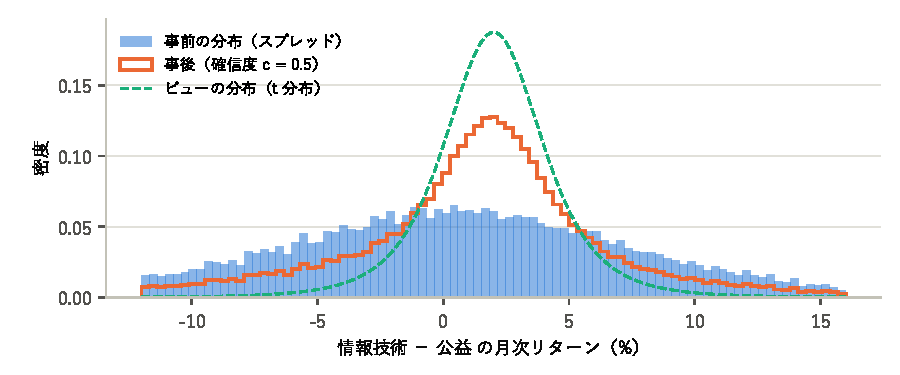
\includegraphics[width=0.92\linewidth]{fig_cop.pdf}
\caption{情報技術 $-$ 公益のスプレッドの、事前の分布、ビューの分布、COP の事後の分布（確信度 0.5）。}
\label{fig:cop}
\end{figure}

\begin{table}[htbp]
\centering
\caption{COP と市場版の BL の、各セクターの期待リターンの変化（月次 \%）。市場版の BL は、スプレッドの平均を COP の事後の平均と同じ値にする条件を付けたもの。}
\label{tab:cop}
\tabin{cop}
\end{table}

結果は次のとおりである（\figref{fig:cop}、\tabref{tab:cop}）。

\begin{itemize}
\item スプレッドの平均は \V{cop.m0}\% から \V{cop.m1}\% に、標準偏差は \V{cop.sd0}\% から \V{cop.sd1}\% になった。事後の分布は、事前の広い分布とビューの尖った分布の混合で、中心が尖り、裾は事前の厚さを残す。5\% 点は \V{cop.q05.0}\% から \V{cop.q05}\% に、95\% 点は \V{cop.q95.0}\% から \V{cop.q95}\% に縮んだ。
\item 期待リターンが動いたのは、情報技術（$+$）と公益（$-$）だけで、ほかのセクターの変化は最大 \V{cop.otherdiff}\% だった。補う行をビューに直交させたので、ほかの方向の変数がそのまま残ったためである。
\item 市場版の BL で同じ大きさの平均の変化を入れると、相関を通じてほかのセクターも動く（情報技術と相関の高い一般消費財や資本財は上がり、公益に近い生活必需品や不動産は下がる）。
\end{itemize}

COP と BL のどちらの動き方が正しい、ということはない。「ほかの資産には何も言っていない」と考えるなら COP のように動かさず、「ほかの資産も、相関に応じて同じ情報の影響を受けるはず」と考えるなら BL のように動かす。COP では補う行の選び方で、この振る舞いを選べる。エントロピー・プーリングでは、平均だけを条件にすれば BL に近い動き方になる（\chapref{ch:ep}）。

\section{正規分布でない市場での BL の研究}

\begin{paperbox}[Giacometti, Bertocchi, Rachev and Fabozzi（2007）, \textit{Stable distributions in the Black--Litterman approach to asset allocation}, Quantitative Finance 7(4)]
均衡の議論を、裾の厚い安定分布の市場に拡張した（Meucci 2010 による紹介）。BL のビューを、裾のリスクの指標（VaR、CVaR）の計算に入れる方法も論じている。
\end{paperbox}

\begin{paperbox}[Teplova, Mikova, Munir and Pivnitskaya（2023）, \textit{Black-Litterman model with copula-based views in mean-CVaR portfolio optimization framework with weight constraints}, Economic Change and Restructuring 56(1)]
\begin{itemize}
\item 10 の国際的な ETF の日次データ（2012〜2022 年）。
\item ARMA-GARCH とコピュラから作った期待リターンを投資家のビューの代わりに使い、リスクは CVaR で測る。多変量のつながりは、柔軟な R-vine コピュラで表す。
\item コピュラに基づく BL（CBL）、コピュラ-CVaR、平均分散、等金額を、比率の上限 30\%、40\%、50\% のもとで、標本外で比べる。ビューへの確信のパラメータ $\tau$ も変える。
\item CBL は裾のリスクが小さく、リスク調整後のリターンが高かった。コピュラ-CVaR は回転率と損益分岐点で優れていた。$\tau$ の値は結果に大きく効いた。
\end{itemize}
\end{paperbox}

\begin{itemize}
\item Alpern と Rachev（2025）は、BL で期待リターンを作り、リスクは多変量のアフィン一般化双曲型分布（正規逆ガウス分布）で CVaR として測った（\chapref{ch:esg}）。
\item 株式のリターンを正規分布の混合で表し、市場の均衡を逆最適化で取り込み、CVaR を最小にする研究もある（\textit{Incorporating Black-Litterman Views in Portfolio Construction when Stock Returns are a Mixture of Normals}, arXiv 1706.03287）。
\end{itemize}

これらの研究に共通するのは、「期待リターンは BL（またはビューに基づく方法）で作り、リスクは裾を表せる分布で測る」という分業である。期待リターンの推定の誤差を BL で抑えつつ、正規分布の仮定が最も効く裾のリスクは、別のモデルに任せる。

\begin{tipbox}[コツ：正規分布でない市場]
\begin{enumerate}
\item 期待リターンは BL で、裾のリスクは $t$ 分布やコピュラのシナリオで、と分けて考える。
\item 暴落のときの連動（裾の依存）を表したいなら、正規分布のコピュラではなく、$t$ コピュラや vine コピュラを使う。
\item COP では、ビューに含まれない資産をどう動かすか（補う行の選び方）を意識して決める。
\item ビューを分布で言えるのが COP の利点である。裾の厚いビューや非対称なビューを入れたいときに使う。
\end{enumerate}
\end{tipbox}

\begin{keybox}[この章のまとめ]
\begin{itemize}
\item COP は、ビューの変数の分布を、事前の分布と主観的な分布の混合に置き換え、コピュラ（順位のつながり）は保つ。
\item 例では、スプレッドの分布は中心が尖り、裾の厚さは残った。補う行をビューに直交させると、ほかの資産は動かない。
\item 正規分布でない市場での BL の研究は、期待リターンを BL で作り、リスクを裾の厚い分布や CVaR で測る、という分業をとるものが多い。
\end{itemize}
\end{keybox}
